کد مورد نظر در زیر آمده‌است. مطابق کد، برای حل مساله از تابع
\lr{solve\_with\_removed\_index}
استفاده می‌شود که با حذف تعدادی از واکنش‌ها، مساله‌ی بهینه‌سازی را تشکیل داده و حل می‌کند. خروجی برنامه در شکل
\ref{fig:q3}
قابل مشاهده است (اعداد در این شکل آورده شده‌اند).\\
در توضیح بخش ب: مشخص است که یکی از با حذف یک دسته‌از از آزمایش‌ها، نرخ فرق چندانی نمی‌کند اما با حذف یک دسته‌ی دیگری، فرق زیادی می‌کند. علتش این است که همانطور که توضیح داده شده است، هر آزمایش به تعدادی مواد نیاز دارد که دیگری آزمایش‌ها آن را برایش فراهم می‌کنند چون $Sv=0$. در نتیجه از نتیجه‌ی حاصل می‌توان دید که یکی از آزمایش‌ها تاثیر زیادی (چه مستقیم و چه غیرمستقیم) در فراهم کردن مواد لازم برای آزمایش \lr{biomass} داشته و به شدت ضروری بوده است در حالی که‌ آزمایش دیگر این‌گونه نبوده است. به طور دقیق‌تر
\lr{transport}
بسیار ضروری بوده است چون با حذف آن نرخ بهینه به شدت کاهش پیدا کرده است.
\lstset{language=Python}
\begin{latin}
\lstinputlisting[breaklines]{../code/q3.py}
\end{latin}
\begin{figure}[H]
	\centering
	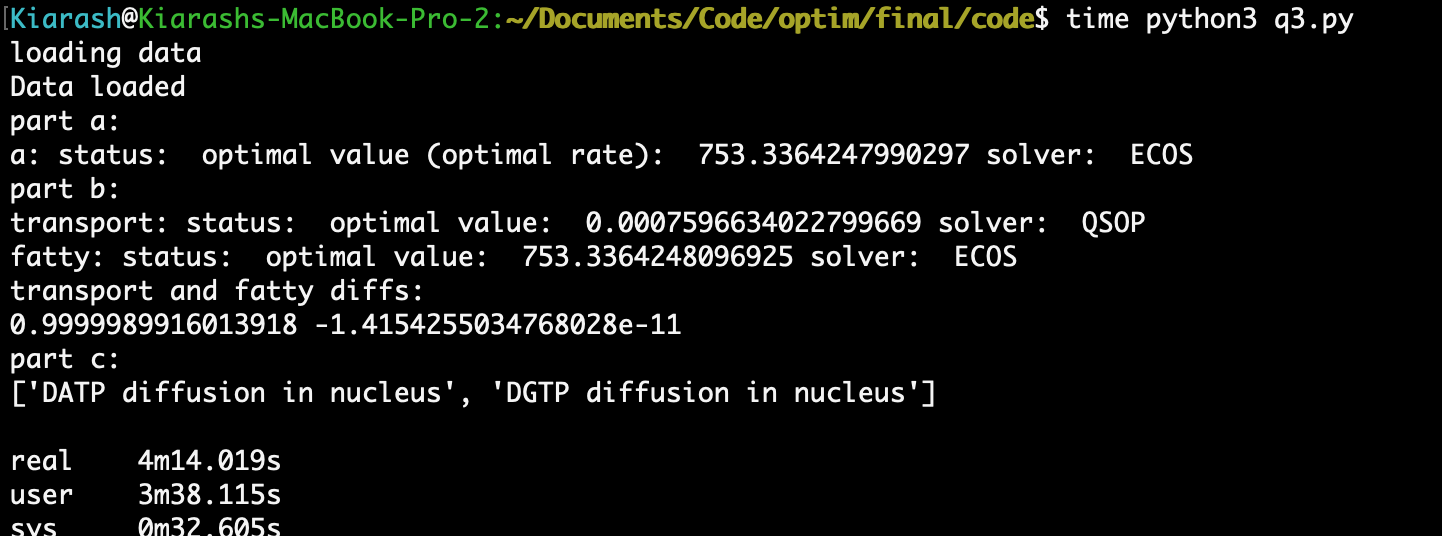
\includegraphics[width=0.9\textwidth]{q3}
	\caption{شکل سوال ۳}
	\label{fig:q3}
\end{figure}